\documentclass{standalone}
\usepackage{amsmath}
\usepackage{tikz}
\begin{document}
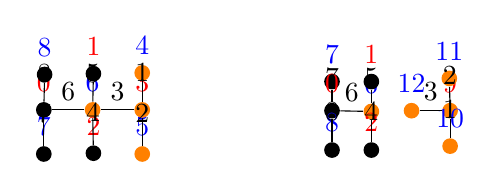
\begin{tikzpicture}
\node[fill=orange, circle, inner sep=2pt, label=above:{\textcolor{blue}{$5$}}] (G1N5) at (4.39,-4.05) {};
\node[fill=orange, circle, inner sep=2pt, label=above:{\textcolor{red}{$3$}}] (G1N3) at (4.39,-3.49) {};
\node[fill=orange, circle, inner sep=2pt, label=above:{\textcolor{blue}{$6$}}] (G1N6) at (3.76,-3.49) {};
\node[fill=black, circle, inner sep=2pt, label=above:{\textcolor{red}{$0$}}] (G1N0) at (3.14,-3.49) {};
\node[fill=black, circle, inner sep=2pt, label=above:{\textcolor{blue}{$8$}}] (G1N8) at (3.15,-3.04) {};
\node[fill=orange, circle, inner sep=2pt, label=above:{\textcolor{blue}{$4$}}] (G1N4) at (4.39,-3.02) {};
\node[fill=black, circle, inner sep=2pt, label=above:{\textcolor{red}{$1$}}] (G1N1) at (3.77,-3.03) {};
\node[fill=black, circle, inner sep=2pt, label=above:{\textcolor{red}{$2$}}] (G1N2) at (3.77,-4.04) {};
\node[fill=black, circle, inner sep=2pt, label=above:{\textcolor{blue}{$7$}}] (G1N7) at (3.14,-4.05) {};
\draw[draw=black, shorten >=0pt, shorten <=0pt] (G1N6) -- (G1N0) node[midway, above] {\textcolor{black}{$6$}};
\draw[draw=black, shorten >=0pt, shorten <=0pt] (G1N6) -- (G1N1) node[midway, above] {\textcolor{black}{$5$}};
\draw[draw=black, shorten >=0pt, shorten <=0pt] (G1N6) -- (G1N2) node[midway, above] {\textcolor{black}{$4$}};
\draw[draw=black, shorten >=0pt, shorten <=0pt] (G1N6) -- (G1N3) node[midway, above] {\textcolor{black}{$3$}};
\draw[draw=black, shorten >=0pt, shorten <=0pt] (G1N0) -- (G1N8) node[midway, above] {\textcolor{black}{$8$}};
\draw[draw=black, shorten >=0pt, shorten <=0pt] (G1N0) -- (G1N7) node[midway, above] {\textcolor{black}{$7$}};
\draw[draw=black, shorten >=0pt, shorten <=0pt] (G1N3) -- (G1N5) node[midway, above] {\textcolor{black}{$2$}};
\draw[draw=black, shorten >=0pt, shorten <=0pt] (G1N3) -- (G1N4) node[midway, above] {\textcolor{black}{$1$}};
\node[fill=black, circle, inner sep=2pt, label=above:{\textcolor{blue}{$7$}}] (G2N7) at (6.8,-3.13) {};
\node[fill=black, circle, inner sep=2pt, label=above:{\textcolor{red}{$0$}}] (G2N0) at (6.8,-3.5) {};
\node[fill=orange, circle, inner sep=2pt, label=above:{\textcolor{blue}{$6$}}] (G2N6) at (7.3,-3.51) {};
\node[fill=black, circle, inner sep=2pt, label=above:{\textcolor{red}{$1$}}] (G2N1) at (7.3,-3.13) {};
\node[fill=black, circle, inner sep=2pt, label=above:{\textcolor{blue}{$8$}}] (G2N8) at (6.8,-4.0) {};
\node[fill=black, circle, inner sep=2pt, label=above:{\textcolor{red}{$2$}}] (G2N2) at (7.3,-4.0) {};
\node[fill=orange, circle, inner sep=2pt, label=above:{\textcolor{red}{$9$}}] (G2N9) at (8.3,-3.5) {};
\node[fill=orange, circle, inner sep=2pt, label=above:{\textcolor{blue}{$10$}}] (G2N10) at (8.3,-3.95) {};
\node[fill=orange, circle, inner sep=2pt, label=above:{\textcolor{blue}{$11$}}] (G2N11) at (8.29,-3.09) {};
\node[fill=orange, circle, inner sep=2pt, label=above:{\textcolor{blue}{$12$}}] (G2N12) at (7.81,-3.5) {};
\draw[draw=black, shorten >=0pt, shorten <=0pt] (G2N0) -- (G2N6) node[midway, above] {\textcolor{black}{$6$}};
\draw[draw=black, shorten >=0pt, shorten <=0pt] (G2N0) -- (G2N7) node[midway, above] {\textcolor{black}{$7$}};
\draw[draw=black, shorten >=0pt, shorten <=0pt] (G2N0) -- (G2N8) node[midway, above] {\textcolor{black}{$8$}};
\draw[draw=black, shorten >=0pt, shorten <=0pt] (G2N6) -- (G2N1) node[midway, above] {\textcolor{black}{$5$}};
\draw[draw=black, shorten >=0pt, shorten <=0pt] (G2N6) -- (G2N2) node[midway, above] {\textcolor{black}{$4$}};
\draw[draw=black, shorten >=0pt, shorten <=0pt] (G2N9) -- (G2N10) node[midway, above] {\textcolor{black}{$1$}};
\draw[draw=black, shorten >=0pt, shorten <=0pt] (G2N9) -- (G2N11) node[midway, above] {\textcolor{black}{$2$}};
\draw[draw=black, shorten >=0pt, shorten <=0pt] (G2N9) -- (G2N12) node[midway, above] {\textcolor{black}{$3$}};
\end{tikzpicture}
\end{document}
